\documentclass[11pt,conference]{IEEEtran}
%\usepackage[utf8x]{inputenc}
\usepackage[dvips]{hyperref}
\usepackage{amssymb}
\usepackage{amsmath}
\usepackage{amsfonts}
\usepackage{amsthm}
\usepackage{algorithm}
\usepackage{subfigure}
\usepackage{graphicx}
\usepackage{bigstrut}
\usepackage{algpseudocode}
\usepackage{framed}
\usepackage{color}
\usepackage{multirow}
\usepackage{cite}
\usepackage{footnotetext}
\usepackage{mcode}

\voffset 20pt

% Title Page
\title{Compressed Sensing for MRI Reconstruction}
\author{Shree Ranga Raju N. M.\\
Department of Systems Design Engineering, \\
University of Waterloo, Waterloo, Ontario, Canada - N2L 3G1 \\
Email : srrajuna@uwaterloo.ca}


\begin{document}
\maketitle

\begin{abstract}
Compressed sensing (CS) is a novel paradigm of signal recovery and sampling that allows signal acquisition using fewer measurements than that of traditional Nyquist-Shannon sampling theorem whenever the signal is sparse. This leads CS to have greater ability in reducing data acquisition time in MRI. In conventional CS-MRI methods, an image is reconstructed by using its sparse representation with respect to a certain basis (Cosine and Wavelet). In recent years, a numerous algorithms have been developed for recovering sparse signals. In this paper, we introduce a novel sparse recovery algorithm called Gini Index based Backtracking Adaptive Orthogonal Matching Pursuit (GI-BAOMP) which is a variation of BAOMP algorithm for image reconstruction. GI-BAOMP is an adaptive greedy algorithm which does not require a prior knowledge of the sparsity level. MATLAB experiments are carried out for Discrete Cosine Transform (DCT) and Discrete Wavelet Transform (DWT) sparse domain. Reconstructed image quality is measured by calculating the Peak signal to Noise Ratio (PSNR).
\end{abstract}

\section{Introduction}
Magnetic Resonance Imaging (MRI) is one of the important modalities used today in the field of Medical Imaging. Compared to other modalities like X-ray and Computer Tomography (CT), MRI has an advantage in imaging soft tissues and it does not require ionizing radiations. Despite of all the advantages, some of the major problems are inevitable. MRI is very expensive and relatively long imaging time of MRI remains as one of the greatest challenges for clinical operations, often limiting its application. 

\par In recent years, Compressed Sensing (CS) introduced by Donoho and Candes \cite{dld,ejt} emerged as a novel paradigm for data acquisition. It senses the data in a rate much lower than the traditional Nyquist rate. It is expected to answer one of the issues in MR image acquisition i.e., fast imaging time acquisition without loosing its quality. It is based on the idea that the signal (image) has sparse representation in a known a priori basis. A signal, $\mathbf{x}$ of length $N$ can be transformed into an orthogonal basis like Wavelet, Cosine or Fourier. The transformed signal has a sparse representation that has at most $K$ ($K$ $<<$ $N$) number of non-zero values. Sparse signals are recovered using sparse signal recovery algorithms. These algorithms can be broadly classified into three main categories: 1) Convex optimization methods. It includes algorithms like Basis Pursuit ($l_1$ norm minimization)\cite{sdma} etc. These type of algorithms are slow, but require less number of measurements\cite{et,sdma}. 
Also, these methods show elegant theoretical guarantees, but the computational complexity is very high, which makes them impractical for most real world application. 2) Greedy pursuit algorithms. Greedy algorithms are fast, but requires more measurements for optimal signal recovery and also they need a priori knowledge about the sparsity level(number of non-zero coeffecients in a sparse signal). These algorithms received significant popularity due to their simple geometric interpretation and low computational complexity. Prominent ones include Orthogonal Matching Pursuit (OMP)\cite{omp}, Regularized OMP (ROMP) \cite{romp}, Stagewise OMP (StOMP) \cite{stomp}, Subspace Pursuit (SP)\cite{sp}, and Compressive Sampling Matching Pursuit (CoSaMP) \cite{cosamp}. 3) Adaptive greedy pursuit algorithms. These are similar to greedy pursuits, however they do not require a prior knowledge about the sparsity level which is the case in most practical applications. These include Backtracking Adaptive Matching Pursuit (BAOMP)\
cite{baomp}, Forward backward pursuit (FBP)\cite{fbp}, etc.
 
\par Lustig et al in \cite{lustig} showed that MR image is suitable for CS implementation because they have sparse representation in certain transformation domain. \cite{lustig} claims that the Discrete Cosine Transform (DCT) and Discrete Wavelet Transform (DWT) have shown good performance in recovering MR images with only 5-10 $\%$ coefficients. However, it is believed that the success of reconstruction does not only merely depend upon the sparse representation of the signal. It also depends on the type of measurement matrix, the statistical properties of the signal, and other parameters. For instance, \cite{circulant} shows sparse signal recovery using circulant matrices. Also, MRI reconstruction using Double-Density Dual tree Discrete wavelet transform can be found in \cite{dualtree}.  

\par In this report, we propose a novel algorithm for sparse signal recovery which is known as Gini Index based Backtracking Adaptive Orthogonal Matching Pursuit (GI-BAOMP). This algorithm is just a simple modification of Backtracking Adaptive Orthogonal Matching Pursuit (BAOMP) \cite{baomp}. Proposed method is an adaptive algorithm where a prior knowledge about the sparsity level is not required for accurate reconstruction of the signal. We compare the novel method with BAOMP algorithm under DCT and DWT domain  of brain MRI image.
\par The rest of the report is organized as follows. In section \ref{sec:mr}, MRI, CS, and sparse recovery algorithms have been discussed briefly. Experiments and results are described in section \ref{sec:exp}. Finally, conclusions and future work is given in section \ref{sec:last}. 



\section{MRI, CS, and GI-BAOMP}
\label{sec:mr}
\subsection{Magnetic Resonance Imaging (MRI)}
MRI signals are generated by the protons present in the hydrogen atoms, which is a main component of human body. Each and every proton in an hydrogen atom nucleus possesses a fundamental spin. As they are positively charged particles, when human body is subjected to a strong static magnetic field $B_0$, protons will align themselves within the magnetic field resulting to a net magnetic moment precessing around $B_0$. This magnetic precession is known as Lamor precession. Its frequency is directly proportional to the applied magnetic field strength which is defined by the following equation
\begin{equation}
 f = \gamma B_0
\end{equation}
where $\gamma$ is a constant. Next, a radio frequency (RF) pulse is applied perpendicular to $B_0$. If the frequency of the applied pulse is equal to the Lamor frequency, the net magnetic moment will be tilted away. Once the applied RF signal is removed, the protons realign themselves such that the net magnetic moment is again aligned around $B_0$. The protons return to the equilibrium by releasing out the RF signal, which is then captured by the conductive field. This measure collects data in the frequency domain (k-space) and this process is called image acquisition. Because of various physical and physiological constraints, most MRI imaging techniques use a sequence of acquisitions and each one samples a part of k-space. Furthermore, this collected data is converted to gray scale images. More descriptions of MRI can be found in the survey paper by Wright \cite{wright}.

\subsection{Compressed Sensing (CS)}
MRI obeys two most prominent requirements for successful application of CS\cite{csmri}: 1) Medical images are naturally compressible by sparse coding in an appropriate transform domain (e.g., by wavelet or cosine transform), and 2) MRI scanners naturally acquire encoded samples, rather than direct pixel samples.

\par There are three stages in CS scheme. a) Encoding: It is a stage of sparsifying input signal (image) using a certain basis such as Fourier, Cosine or Wavelets. b) Sensing: This phase is a process to measure the sparse signal representation and reduce its dimension using measurement (sensing) matrix. c) Decoding: This is a process of reconstructing the sensed signal.

\par CS has the following frame work. \\
Consider the standard signal acquisition model which acquires a signal, $\mathbf{x} \in \mathbb{R}^N$ via linear measurements using the following equation
\begin{equation}
 \label{Eqn:CS}
 \mathbf{b} = \mathbf{Ax} + \mathbf{w}
\end{equation}  

where $\mathbf{A} \in \mathbb{R}^{M\times N}$ represents a measurement (sensing) matrix, $\mathbf{b} \in \mathbb{R}^M$ represents the measurement vector, and $\mathbf{w} \in \mathbb{R}^M$ represents the additive measurement noise in the system.

\par In CS framework, we have, $M<<N$ which makes equation (1) an ill-posed problem i.e., to solve an under determined system of linear equations. However, T. Tao et al. in \cite{ejt} proposed that with the additional knowledge of signal (image) being $K$-sparse (at most $K$ non-zero values, and $K$ $<$ $M$) when transformed to the sparse domain, we can uniquely recover the image using sparse recovery algorithms. In this paper, we use Backtracking Adaptive Orthogonal Matching Pursuit algorithm to recover the sparse signal.


\subsection{Gini Index - Backtracking Adaptive Orthogonal Matching Pursuit (GI-BAOMP) }

\par In this report, we propose a novel algorithm called Gini Index-based Backtracking Adaptive Orthogonal Matching Pursuit(GI-BAOMP) for sparse reconstruction. It is a modification of BAOMP algorithm (BAOMP) \cite{baomp}. BAOMP algorithm for sparse signal recovery was introduced by Huang et al. as shown in Algorithm \ref{alg:BAOMP} in \cite{baomp}. Proposed algorithm makes use of Gini Index (GI) \cite{GI} as a tool to choose the atoms initially to form the candidate set and also to form the atoms deletion set. The algorithm is described in Algorithm \ref{alg: gi-baomp}

\begin{algorithm}
 \caption{Backtracking Adaptive Orthogonal Matching Pursuit (BAOMP)}
\label{alg:BAOMP} 
{\bf Input:} \\
$\mathbf{A}_{M \times N}$ - measurement matrix\vspace{0.3cm} \\
 $\mathbf{b}_{M \times 1}$ - sampled measurement vector\vspace{0.3cm} \\
 $\mu_1$ - a preset atom adding constant threshold in [0,1]\vspace{0.3cm} \\
 $\mu_2$ - a preset atom deleting constant threshold in [0,1]\vspace{0.3cm} \\
maxiter - Maximum number of iterations\vspace{0.3cm} \\
 $\varepsilon$ = Convergence threshold to stop the iterations. \vspace{0.1cm} \\
\begin{algorithmic}
\State Initialize: $\mathbf{x}^0$ = 0 (initial solution), $\mathbf{r}^0$ = $\mathbf{b}$ (initial residual), $\Delta$ = $\emptyset$ (estimated support, empty at the begining), $\lambda^0 = \emptyset$ (candidate set), $\Gamma^0 = \emptyset$ (delete set).
\Repeat
\State n = 1;
\State $\mathbf{u}$ = $\mathbf{A}^T \mathbf{r}^{n-1}$;
\State $L^n$ = $\mu_1 times |\mathbf{u}|$;
\State $\lambda^n$ = indices of $L^n$ elements of $\mathbf{u}$ with highest magnitudes.
\State $\mathbf{x}^n_{\Delta \cup \lambda^n}$ = $\mathbf{A}^\dagger_{\Delta \cup \lambda^n} \mathbf{b}$;
\State $\Gamma^n$  = Select atoms such that $|\mathbf{x}^n_{\Delta \cup \lambda^n}| <$ $\mu_2$ $times$ max$|\mathbf{x}^n_{\Delta \cup \lambda^n}|$
\State $\Delta$ = $\{\Delta \cap \lambda^n\} \setminus \Gamma^n$;
\State $\mathbf{x}_\Delta^n$ = $\mathbf{A}^\dagger_\Delta \mathbf{b}$;
\State $\mathbf{r}^n$ = $\mathbf{b} - \mathbf{A}_\Delta \mathbf{x}^n_\Delta$;
\Until ($\|\mathbf{r}^n\|_2 < \varepsilon$) or (n == maxiter)
\State n = n + 1; 
\end{algorithmic}
{\bf Output:} $\Delta, \mathbf{x}_\Delta^n$ = $\mathbf{A}^\dagger_\Delta \mathbf{b}$, $\mathbf{x}^n_{\Delta^c} = 0$.
\end{algorithm}


\par Before describing the GI-BAOMP algorithm, a brief overview about a few existing greedy algorithms like OMP \cite{omp}, SP \cite{sp}, BAOMP \cite{baomp}, and FBP \cite{fbp} is given.

\par In these algorithms, the sensing matrix $\mathbf{A}$ is considered as a dictionary with each column vector $\Phi_i$ as an atom. In oder to recover sparse signal from equation \eqref{Eqn:CS}, each iteration consists of two major steps. 1) Atom selection step i.e., to find one or several atoms which have the largest correlation with the residue and adding them to the support set $T$. 2) Update the approximation $\mathbf{x}_T$ to minimize the new residual error i.e., min$\|\mathbf{b}-\mathbf{A}_T\mathbf{x}_T\|$ and then update the residue. 


\begin{figure*}
\begin{center}
\subfigure[]{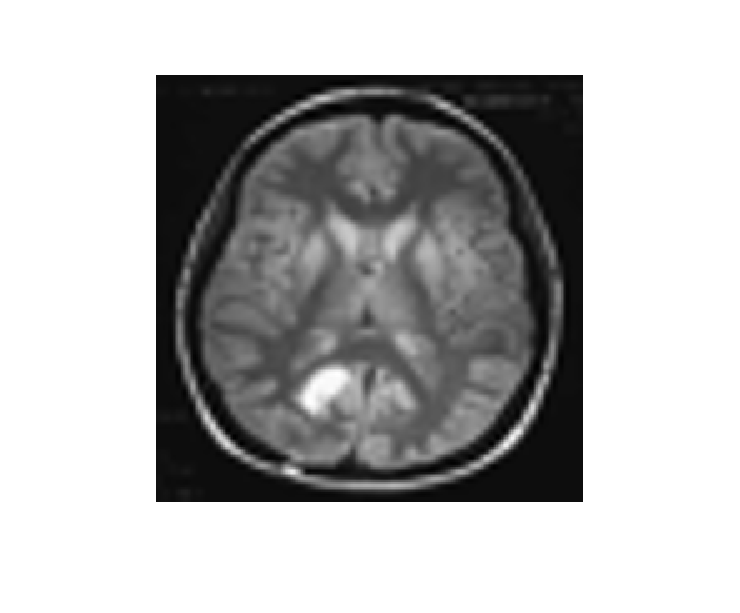
\includegraphics[width=1.5in,height=1.5in]{Experiments/orig.eps}}
\hspace{-0.4in} %\vspace{-0.15in}
\subfigure[]{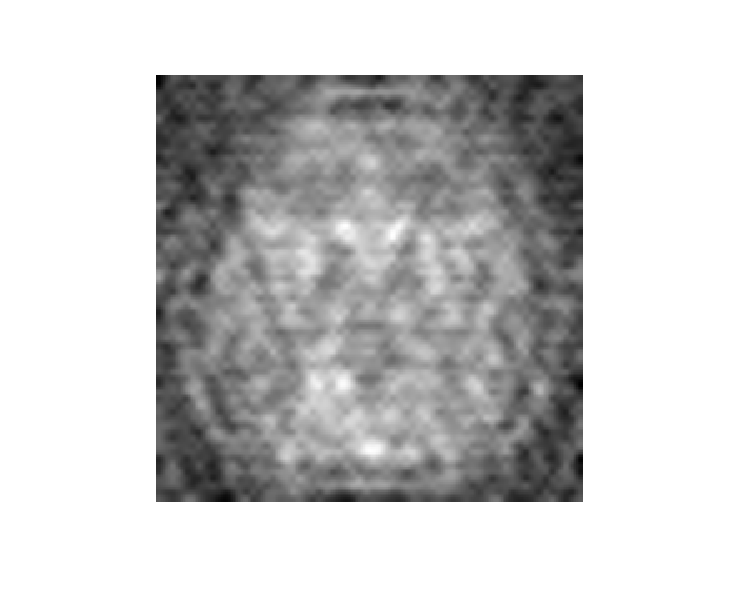
\includegraphics[width=1.5in,height=1.5in]{Experiments/DCT_BAOMP_0.3.eps}}

\subfigure[]{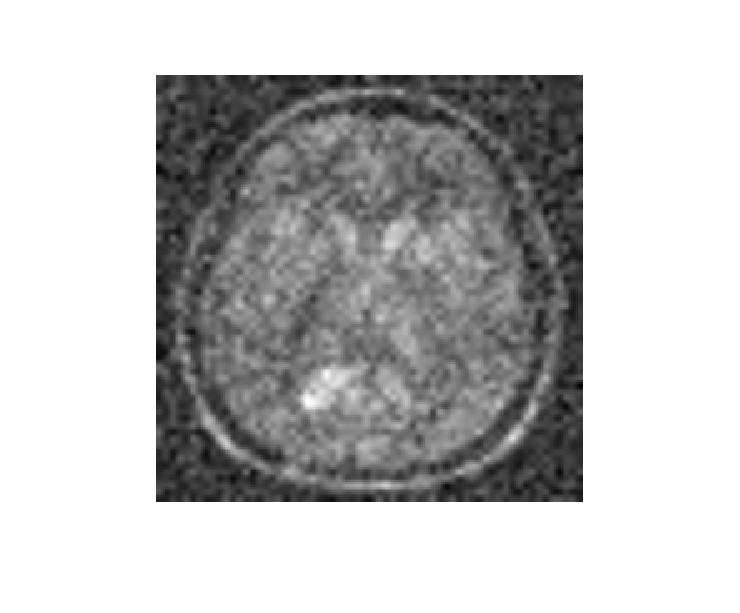
\includegraphics[width=1.5in,height=1.5in]{Experiments/DCT_BAOMP_0.6.eps}}
\hspace{-0.4in} %\vspace{-2.5in}
\subfigure[]{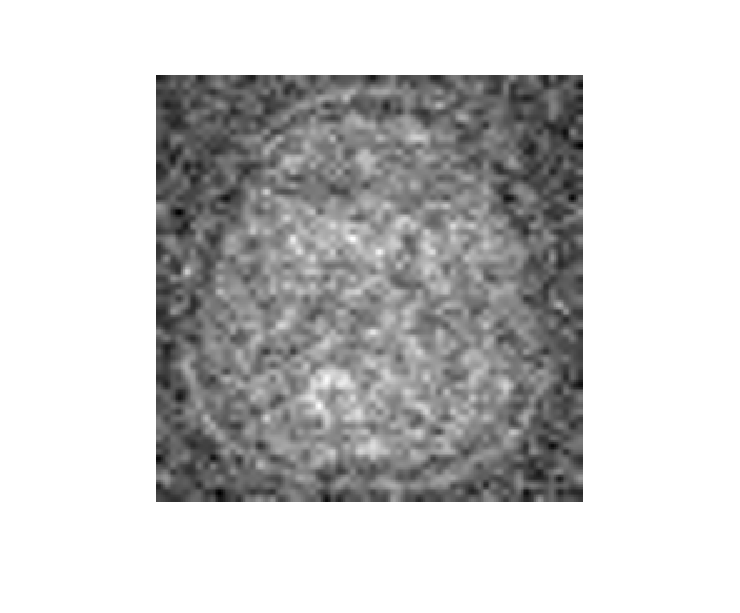
\includegraphics[width=1.5in,height=1.5in]{Experiments/DCT_BAGIOMP_0.3.eps}}
\hspace{-0.4in}
\subfigure[]{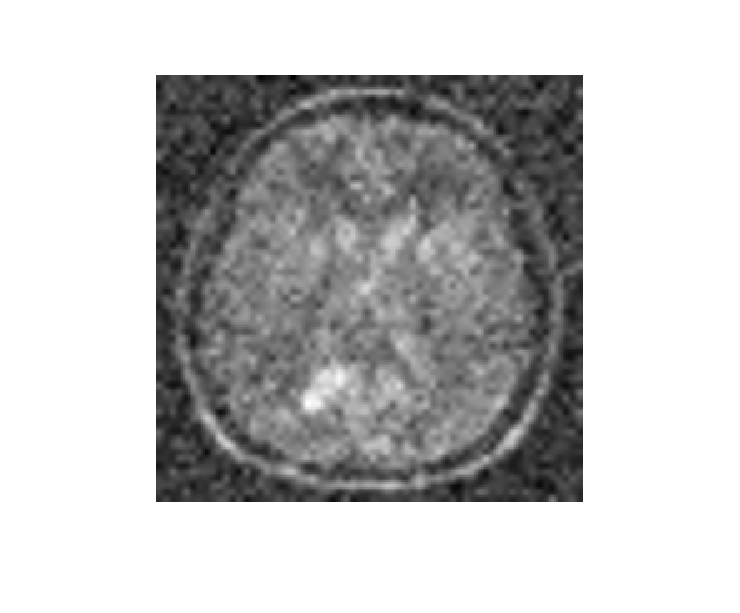
\includegraphics[width=1.5in,height=1.5in]{Experiments/DCT_BAGIOMP_0.6.eps}}
 
\end{center}
\caption{(a) is the original Brain MRI image. (b) is the reconstructed image from BAOMP under DCT sparse domain with 30\% measurements. (c) is the reconstructed image from BAOMP under DCT sparse domain with 60\% measurements. (d) is the reconstructed image from GI-BAOMP under DCT sparse domain with 30\% measurements. (e) is the reconstructed image from GI-BAOMP under DCT sparse domain with 60\% measurements.}
\end{figure*}



\par OMP \cite{omp} chooses one prominent atom in each iteration that gives maximum correlation between the columns of measurement or sensing matrix and the residual. Once the coordinate atoms are selected, they will remain in the process till the end and they cannot be removed. This might lead to an unreliable sparse reconstruction if wrong supports have been chosen. Unlike OMP, SP \cite{sp} and CoSaMP (similar to SP) \cite{cosamp} select $K$ or 2$K$ coordinates and uses an iterative check to refine the performance of sparse signal recovery. However, SP and CoSaMP require a prior knowledge of sparsity level for exact reconstruction. In practical applications this information is not available and hence, other adaptive greedy methods like BAOMP \cite{baomp}, FBP \cite{fbp} were proposed for sparse signal recovery. Most of the adaptive algorithms make use of threshold based approach. For instance, BAOMP uses a threshold parameter $\mu_1$ which has a range of 0.4 - 0.8 to adaptively choose several atoms at each 
iteration initially to form the candidate set, then uses another parameter $\mu_2$ that also has a range of 0.4 - 0.8 to form the atom deletion set and then incorporates a simple backtracking strategy similar 
to that of SP and CoSaMP to remove atoms chosen incorrectly in the previous iteration, to form the support set more accurately. In a similar manner, FBP uses a threshold parameter $\alpha$ to form the search space dimension and $\beta$ to form the atom delete set and then incorporates backtracking method. Also in \cite{fbp}, we can see that experiments have been performed for different values of $\alpha$ and $\beta$ chosen. However, parameters like $\alpha$, $\beta$, $\mu_1$ etc are heuristic. Therefore, for a given signal, one might not be able to decide on specific values in the given range to be chosen to obtain the best sparse signal reconstruction. In oder to alleviate that, GI-BAOMP method as shown in Algorithm \ref{alg: gi-baomp} is proposed in which GI \cite{GI} based thresholding approach is used to form the atoms selection and the atom delete set.

\begin{figure*}
\centering
\subfigure[]{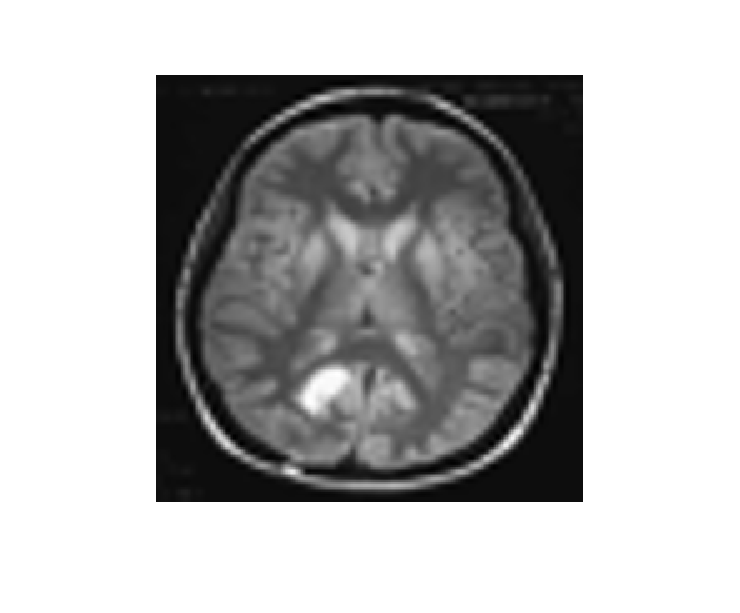
\includegraphics[width=1.5in,height=1.5in]{Experiments/orig.eps}}
%\hspace{-1.5in} %\vspace{-0.5in}
\subfigure[]{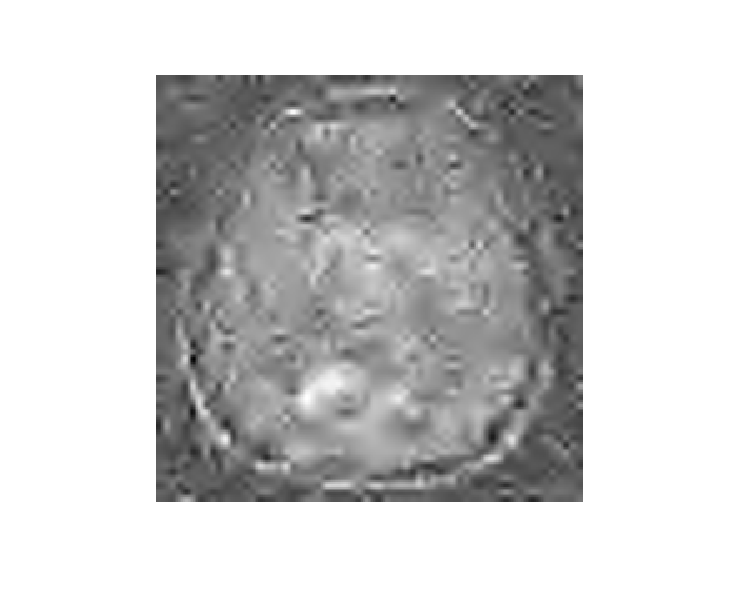
\includegraphics[width=1.5in,height=1.5in]{Experiments/DWT_BAOMP_0.3.eps}}

\subfigure[]{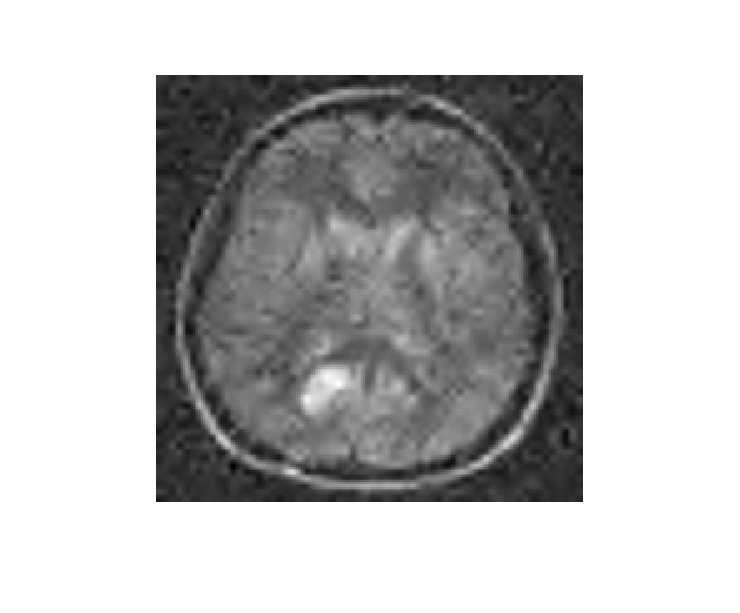
\includegraphics[width=1.5in,height=1.5in]{Experiments/DWT_BAOMP_0.6.eps}}
%\hspace{-1.5in} %\vspace{-2.5in}
\subfigure[]{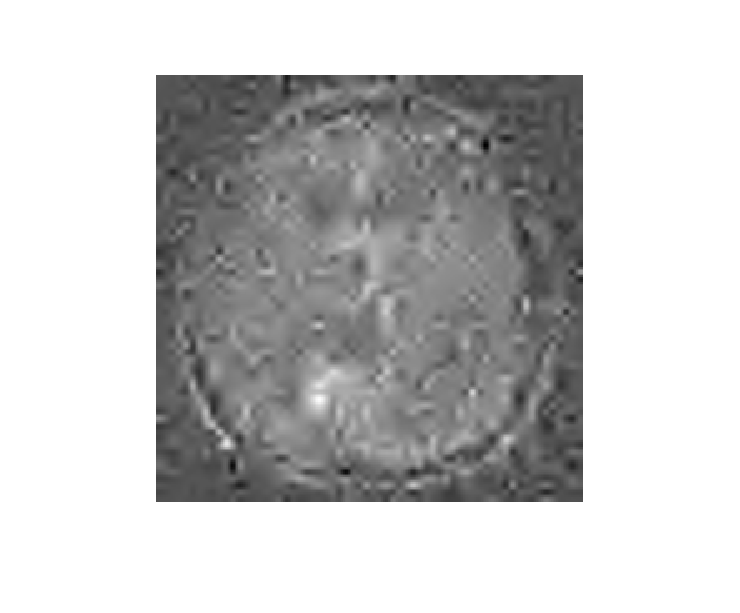
\includegraphics[width=1.5in,height=1.5in]{Experiments/DWT_BAGIOMP_0.3.eps}}
\subfigure[]{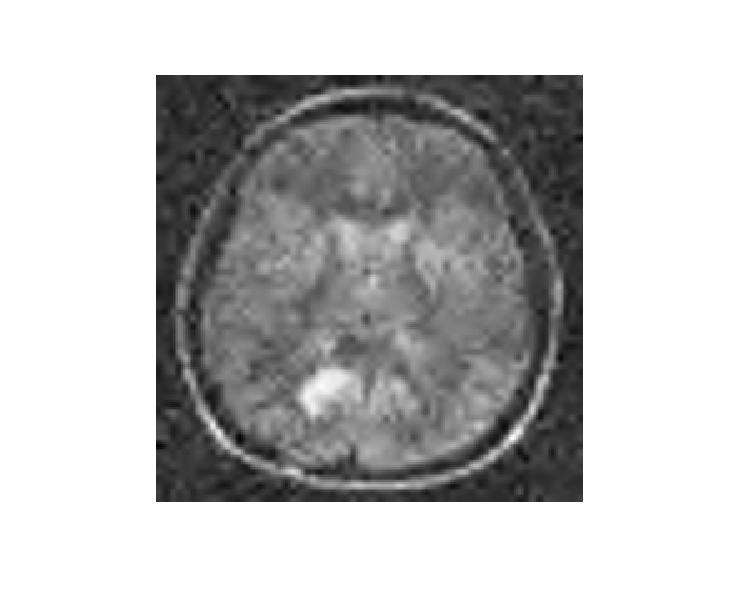
\includegraphics[width=1.5in,height=1.5in]{Experiments/DWT_BAGIOMP_0.6.eps}}
\caption{(a) is the original Brain MRI image. (b) is the reconstructed image from BAOMP under DWT sparse domain with 30\% measurements. (c) is the reconstructed image from BAOMP under DWT sparse domain with 60\% measurements. (d) is the reconstructed image from GI-BAOMP under DWT sparse domain with 30\% measurements. (e) is the reconstructed image from GI-BAOMP under DWT sparse domain with 60\% measurements.}
\end{figure*}

\begin{algorithm}
 \caption{Gini Index based BAOMP (GI-BAOMP)}
\label{alg: gi-baomp}
{\bf Inputs:} $\mathbf{A}_{M \times N}$, $\mathbf{b}_{M \times 1}$, maxiter = Maximum number of iterations, and $\varepsilon$ = Convergence threshold to stop the iterations.
\begin{algorithmic}
\State Initialize: $\mathbf{x}^0 = 0$, $\mathbf{r}^0 = \mathbf{b}$, 
\State $T = \emptyset$ (Final Set. Empty at the beginning) 
\State $C^0 = \emptyset$ (Candidate Set) 
\State $D^0 = \emptyset$ (Delete Set) 
\State $n = 1;$ 
\Repeat
\State $C^n$ = find the indices which satisfies, \\ \hspace{1.6cm} $|<\mathbf{r}^{n-1},$ $\Phi_{C^n}>|$ $\geq$ GI($\mathbf{r}^{n-1}$) . max$_{j\in \Psi} |<\mathbf{r}^{n-1},\Phi_{j}>|$, \\ \hspace{1.6cm}$\Psi$ = [1,2,3,...,N]. %and with $|C^n | \leq M - |T|$
%\State $T = T \cup C^n;$
\State $\mathbf{x}_{T \cup C^n}^n = \mathbf{A}^\dagger_{T \cup C^n}  \mathbf{b};$
\State $D^n$ = choose indices such that it satisfies, \\ \hspace{1.6cm} $|\mathbf{x}^n_{T \cup C^n}|$ $<$ GI$(\mathbf{x}^n_{T \cup C^n})$ . max$|\mathbf{x}^n_{C^n}|$
\State $T = (T \cap C^n) \setminus D^n;$
\State $\mathbf{x}_T^n = \mathbf{A}^\dagger_T  \mathbf{b};$
\State $\mathbf{r}^n = \mathbf{b} - \mathbf{A}_T \mathbf{x}_T^n;$
\Until($\|\mathbf{r}^n\|_2 < \varepsilon$) or (n == maxiter)
\State $n = n + 1;$
\end{algorithmic}

{\bf Output:} $T, \mathbf{x}_T = \mathbf{A}^\dagger_T  \mathbf{b}$, and $\mathbf{x}_{T^c} = 0$
\end{algorithm}


\par From Algorithm \ref{alg: gi-baomp}, $T$ is the estimated support set until the current iteration, and matrix $\mathbf{A}_T$ consists of the columns of $\mathbf{A}$ with coordinates listed in $T$. Like most greedy pursuit algorithms, the first step of the proposed method is to select the candidate set $C^n$ whose correlation between the columns of $\mathbf{A}$ and the residual $\mathbf{r}^{n-1}$ is not less than GI($\mathbf{r}^{n-1}$) . max$_{j\in \Psi} |<\mathbf{r}^{n-1},\Phi_{j}>|$. The GI($\mathbf{r}^{n-1}$) is calculated using the equation \eqref{Eqn:GI}. Here $\Psi$ = [1,2,3,...,N] is the whole coordinate set. GI($\mathbf{r}^{n-1}$) is used to decide the number of atoms to be chosen at each time of the iteration. The output of GI \cite{GI} is always between 0 and 1 for any given vector. If GI is exactly equal to 1, it just chooses the maximum correlation atom each time, similar to that of OMP method. The value of GI output is larger i.e., tending more towards 1 when there are more number of zeroes 
in a given vector. We choose GI of residual to form the search space because residual decreases sequentially as the algorithm converges i.e., the number of zeroes in the residue vector increases, and hence it is more likely that the number of atoms chosen for the next iteration is less. Therefore, GI of residual will be larger (almost equal to 1) making number of atoms chosen for the next iteration less. This avoids choosing a specific number of atoms, unlike SP or CoSaMP, where exactly $K$ or $2K$ number of atoms in each iteration chosen. In the second step of GI-BAOMP algorithm, we remove some of the atoms whose approximate coefficients $\mathbf{x}^n_{T \cup C^n}$ are smaller than GI($\mathbf{x}^n_{T \cup C^n}$) times the maximum amplitude of $\mathbf{x}^n_{C^n}$, where $\mathbf{x}^n_{C^n}$ are the corresponding entries of $\mathbf{x}^n_{T \cup C^n}$ in the current selected set $C^n$ and GI($\mathbf{x}^n_{T \cup C^n}$) is calculated using equation \eqref{Eqn:GI}. This is called backtracking method and it 
has certain intuition. Apparently, the greedy algorithm's ultimate goal is to find the $K$ sparse representation whose approximate coefficients are  $K$ largest and hence to reduce the approximate error sequentially. Ideally, it is expected that approximate coefficients of the previously chosen atoms are larger than that of the currently chosen atoms. At a certain iteration, if the newly chosen atoms make the approximate coefficients of the previously chosen atoms much smaller, it is more likely that these previously selected atoms were chosen incorrectly in the previous iteration. So, GI-BAOMP uses the above backtracking strategy to remove the atoms with relatively small coefficients. Since, $K$ is not one of the input parameter, the proposed method will stop when the $l_2$ norm of the current residual i.e., $\|r^n\|_2$ is less than $\varepsilon$ or when the maximum number of iteration has been reached. 

\par A brief overview of GI is given as follows:

\par Consider a vector, $\mathbf{g}$ = $[\mathbf{g(1),....,g(N)}]^T$, with its elements re-ordered and represented by $\mathbf{g_{[k]}}$
for $\mathbf{k} = 1,2,....,N$, where $\mid\mathbf{g_{[1]}}\mid$ $\leq$ $\mid\mathbf{g_{[2]}}\mid$,....,$\leq$ $\mid\mathbf{g_{[N]}}\mid$, then GI of a vector is given as follows:

\begin{equation}
\label{Eqn:GI}
GI(\mathbf{g}) = 1 - 2 \hspace{0.2cm}\sum^N_{k=1} \frac{\mathbf{g_{[k]}}}{\|\mathbf{g}\|_1} \Big(\frac{N - k + 0.5}{N}\Big)
\end{equation}

where $\|\mathbf{g}\|_1$ is the $l_1$ norm of $\mathbf{g}$.

\par So far, GI has been used as a measure of sparsity \cite{sparsemeasure}. But, in this report we show how GI is used for the purpose of sparse signal reconstruction when there is no a prior information on $K$.

\section{Experiments and Results}
\label{sec:exp}
To demonstrate the effectiveness of GI-BAOMP sparse signal recovery algorithm under DCT and DWT sparse domain, consider a MRI brain image of size 64x64 ($N$ = 4096) as shown in the Figure 1(a). The experiments were carried out on MATLAB R2011b under Ubuntu 12.04 Linux operating system running on Dell XPS Laptop with an intel core i5 processor, 4GB RAM. The intuition behind choosing such a small size image is due to MATLAB memory issues in the laptop. A gaussian random matrix, $\mathbf{A}$ with i.i.d entries of size $M \times N$ was generated as the sensing or measurement matrix. The size of measurement, $M$ is varied as 30 and 60 percentage of $N$. The GI-BAOMP code is written with the parameters mentioned in \cite{baomp} except for the $\mu_1$ and $\mu_2$ parameters. BAOMP algorithm code is written with the parameters as mentioned in \cite{baomp} where $\mu_1$ and $\mu_2$ is set to 0.6. The quality of reconstructed image is measured using Peak-Signal-to-Noise-Ratio (PSNR), which is calculated as given in 
the following equation:

\begin{equation}
 \hat{\lambda} = (\beta_{i,j} - \beta^*_{i,j})^2 
\end{equation}
 where, i = 1,2,...,m 
 and j = 1,2,...,n
\begin{equation}
\varpi = \frac{1}{m\times n}{{\displaystyle\sum_{l=1}^{m\times n}{\hat{\lambda_l}}}}
\end{equation}
where, $\beta$ represents the original image, $\beta^*$ represents the reconstructed image, $'m'$ represents the number of the rows in $\beta$, $'n'$ represents the number of the columns in $\beta$, $\varpi$ represents the Mean square error.
\begin{equation}
 \text{PSNR} = 10 \times log10 (\frac{255^2}{\varpi})
\end{equation}

\begin{table}
\begin{center}
\begin{tabular} {|c|c|c|}
\hline

 Measurements, $M$ & 0.3*$N$ & 0.6*$N$ \\
 \hline
 BAOMP PSNR under DCT domain & 17.36 & 19.16 \\
 \hline
 GI-BAOMP PSNR under DCT domain & 15.25 & 19.70 \\
 \hline
 BAOMP PSNR under DWT domain & 17.18 & 22.90 \\
 \hline
 GI-BAOMP PSNR under DWT domain & 16.17 & 22.80 \\
 \hline
 \end{tabular}
\caption {This table shows the PSNR values for the reconstructed image under DCT and DWT sparse domains for both BAOMP and GI-BAOMP algorithms.}
\end{center}
\end{table}

\par Figure 1. shows the reconstructed images under DCT domain and Figure 2. shows the reconstructed images under DWT domain. Table 1. shows the PSNR values for the reconstructed brain MRI image under different sparse domains for BAOMP and GI-BAOMP algorithms. It can be observed from the table 1. that both the algorithms give similar performance. It is also evident that the DWT is a better sparse domain when compared with DCT domain. However, the reconstruction performance does not only depend on the sparsity domain but on other parameters such as the type of the measurement matrix, the statistical nature of the signal etc. And also, the algorithm is tested for only one set of Gaussian random matrix (measurement matrix) for each value of the measurement. The proposed method hence can be tested for more than one set of random matrix and an average (mean) value of the PSNR can be calculated.  

\section{Conclusion and Future Work}
\label{sec:last}
The experiments conducted show the effectiveness of BAOMP and GI-BAOMP algorithm. The proposed algorithm gives almost similar performance when compared with BAOMP algorithm. However, it has the greatest advantage of not depending upon any heuristic values to form candidate set  and atom deletion set. 

\par In future, the experiments can be carried out under various other sparse domains like biorthogonal wavelets, noiselets etc. Also, other sparse recovery algorithms like FBP, OMP, SP and CoSaMP can be compared with the proposed GI-BAOMP algorithm. In our experiment, Gaussian random matrix has been used because it provides incoherence with any sparse signal and also the number of measurements is minimal. However, it requires a huge memory storage and has high computational complexity. So, other kinds of measurement matrices like circular matrices as given in \cite{circulant}, toeplitz matrices, and noiselets can be used to carry out the experiments.  

\par GI-BAOMP does not have elegant theoretical guarantees and logical deductions similar to SP\cite{sp} and CoSaMP \cite{cosamp} because $K$ is not one of the input parameters to the algorithm. So, obtaining these guarantees is left as an open challenge for the future.

\begin{thebibliography}{60}
\bibitem{dld} D.L. Donoho, ``Compressed Sensing'', \emph{IEEE Transactions on Information Theory}, vol. 52, no. 4, 2006.

\bibitem{ejt} E.Candes, J. Romberg, and T.Tao, ``Robust uncertainty principles: Exact signal reconstruction from highly incomplete frequency
information'', \emph{IEEE Trans. on Inf. Theory}, 2006.

\bibitem{csmri} M. Lustig, D. L. Donoho., Juan M. Santos, J .M. Pauly, ``Compressed Sensing MRI,'' \emph{IEEE signal processing magazine}., March 2008.

\bibitem{wright} G. Wright, ``Magnetic resonance imagin,'' \emph{IEEE signal processing magazine}., vol. 14.,no.1, pp. 56-66, Jan 1997. 

\bibitem{et} E.J. Candes and T. Tao, ``Decoding by linear programming'', \emph{IEEE transactions on Info. theory}, vol.51, no.12, pp 
4203-4215, Dec. 2005.

\bibitem{sdma} Scott S. chen and D.L. Donoho, Michael, and A. Saunders, ``Atomic decomposition by basis pursuit'', \emph{SIAM journal
on scientific computing}, vol.20, pp.33-61, 1998.

\bibitem{syl} Shihao Ji, Ya Xue, and L. Carin, ``Bayesian compressive sensing'', \emph{IEEE transactions on signal processing}, vol.56, no.6
 , pp.2346-2356, june 2008.

\bibitem{db} D.P. Wipf and B.D. Rao, ``Sparse bayesian learning for basis selection'', \emph{IEEE transactions on signal processing}, 
vol.52, pp.2153-2164, Aug. 2004.

\bibitem{lustig} M Lustig, D Donoho, JM Pauly. Sparse MRI: The application of compressed sensing for rapid MR imaging. Magn. Reson. Med. 2007; 58(6): 1182-1195.

\bibitem{romp} D. Needell, R. Vershynin, ``Uniform uncertainity principle and signal recovery via regularised orthogonal matching pursuit,'' \emph{Found. Comp. Maths.}, vol. 9, pp. 317-334, 2009.

\bibitem{stomp} D.L. Donoho, Y. Tsaig, I. Drori, J. C. Starck, ``Sparse solution of underdetermined linear equations by stagewise orthogonal matching pursuit,'' [Online] 2006. http://www.dsp.ece.rice.edu/cs.
  


\bibitem{lgxw} Lina Guo, Xianbin Wen, `` SAR image compression and reconstruction based on compressed sensing'', \emph{Journal of inoformation and computational science}, January 20. 2014.

\bibitem{ljzj} L. Jiying, Z. Jubo, Y. Fengxia, Z. Zenghui, `` Theoretical frameworks of remote sensing systems based on compressed sensing'', \emph{ISPRS TC VII symposium}, July, 2010.

\bibitem{omp} J.A. tropp and A.C. Gilbert, ``Signal Recovery from random measurements via orthogonal matching pursuit'', \emph{IEEE Trans. on Information Theory}
vol. 53, no. 12, pp. 4655 - 4666, dec. 2007.

\bibitem{sp} Wei dai and O. Milenkovic, ``Subspace Pursuit for compressive sensing signal reconstruction'', \emph{IEEE Trans. on Information theory}
vol. 55, no.5, pp 2230 -2249, may 2009.

\bibitem{GI} Corrado Gini, ``Variability and Mutability'', 1912.

\bibitem{sparsemeasure} D. Zonoobi, A.A. Kassim, Y.V. Venkatesh, ``Gini Index as sparsity measure for signal reconstruction from
compressive samples'', \emph{IEEE journals of selected topics n signal processing}, vol.5, no.5, Sep 2011.


\bibitem{cosamp} D. Needell, J.A. Tropp, ``Compressive Sampling Matching Pursuit: Iterative signal recovery from incomplete and inaccurate samples'', \emph{Applied computational Harmo. Analysis}., vol. 26, no. 3, pp. 301-321, May 2009. 

\bibitem{samp} T.T. Do, N. Nguyen, and T.D. Tran, ``Sparsity adaptive matching pursuit algorithm for practical CS'', 
\emph{42nd Asilomar Conference}, Oct. 2008.

\bibitem{baomp} Honglin Huang, and Anamitra Makur, ``Backtracking-based matching pursuit method for sprase signal reconstruction'',
\emph{IEEE signal processing letters}, vol.18, no.7, July 2011.

\bibitem{fbp} N.B. Karahangolu, and H. Erdogan, ``Forward-backward search for compressed sensing signal recovery'', \emph{EUSIPCO}, 2012.

\bibitem{circulant} Windra Swastika, Hideaki Haneishi, ``Compressed Sensing for thoraic MRI witha partial random circular matrices'', \emph{Telkomnika}, March -2012; vol. 10. no. 1, pp. 147-154.

\bibitem{dualtree} Z. Zhu, K. Wahid, P. Babyn, R. Yanf, ``CS based MRI reconstruction using complex double density dual tree DWT'', \emph{Int. Jrnl. Biomedical Imaging } vol. 2013, article ID: 907501.
 

\end{thebibliography}


























\end{document}          
